\documentclass[11pt,a4paper]{article}
\usepackage[utf8]{inputenc}
\usepackage[T1]{fontenc}
\usepackage{amsfonts}
\usepackage[french]{babel}
\frenchbsetup{StandardLists=true} % à inclure si on utilise \usepackage[francais]{babel}
\usepackage{enumitem}
\usepackage{amssymb}
\usepackage{amsmath}
\usepackage[left=2cm,right=2cm,top=2cm,bottom=2cm]{geometry}
\usepackage{multirow}
\usepackage[dvipsnames]{xcolor}

\usepackage[T1]{fontenc}
\usepackage{fouriernc}
\usepackage{graphicx}

\usepackage{setspace}
\singlespacing

\usepackage{pstricks}
\usepackage{xkeyval}
\usepackage{pst-labo}


\usepackage{multicol}
\usepackage{caption}
\usepackage{fancyhdr}
\pagestyle{fancy}
\renewcommand\headrulewidth{1pt}
\fancyhead[L]{Lycée Denis Diderot }
\fancyhead[R]{Classe de TMICRO}
\setcounter{page}{1}\fancyfoot[C]{page \thepage}
\fancyfoot[R]{Année 2025 2026}
\fancyfoot[L]{Alexis RUIZ}
\usepackage{multirow,tabularx,booktabs}
\newcommand{\cadreblanc}[1]{%
\medskip\framebox[\linewidth][c]{%
\rule{0mm}{#1mm}}\par
\medskip}

\usepackage{awesomebox}
\setlength{\aweboxvskip}{0mm}
\usepackage{pifont}
\usepackage{chemmacros}
\chemsetup{modules=all}
\setlength{\columnseprule}{.25mm}



\newcommand*\acocher{\quitvmode{\fboxsep0pt \fboxrule0.8pt \fbox{\vrule height1.8ex depth.1ex width0pt \vrule height0pt depth0pt width1.9ex }}}
\newcolumntype{R}[1]{>{\raggedleft\arraybackslash }b{#1}}
\newcolumntype{L}[1]{>{\raggedright\arraybackslash }b{#1}}
\newcolumntype{C}[1]{>{\centering\arraybackslash }b{#1}}

\newcommand{\defproblem}{\awesomebox[black]{2pt}{\rotatebox{90}{\large{\textbf{Problématique}}}}{black}}
\newcommand{\defconclusion}{\awesomebox[black]{2pt}{\rotatebox{90}{\Large{\textbf{Conclusion}}}}{black}}

\frenchbsetup{StandardLists=true}
\begin{document}



\center \LARGE{Activité 1 - Montrer qu'un son se propage dans un milieu matériel}
\\[0,3cm]

\normalsize

\hrule\
\\[0,2cm]

\flushleft \textbf{NOM :\\
Prénom:\\[0,2cm]
}
\hrule\
\\[0,2cm]

\defproblem{\begin{minipage}{14cm}
{
\begin{center}
\textbf{"Dans l'espace personne ne peut vous entendre crier". \\ 
}
\vspace{0.4 cm}
\end{center}
}
\end{minipage}
}
\vspace{1 cm}
\ding{202} Entend-t-on des sons dans l'espace?
\begin{center}
\begin{multicols}{2}
	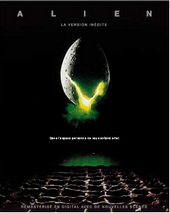
\includegraphics[scale=1]{images/Alien.png} \\
	\cadreblanc{72}
\end{multicols}
\end{center}

\ding{203} Proposer une expérience permettant de confirmer votre hypothèse. 
\renewcommand{\arraystretch}{1}
\begin{tabular}{|p{5cm}||p{11 cm}|}
\hline Matériel & Schéma de l'expérience \\
  &  \\
  &  \\
    &  \\
  &  \\
   &  \\
  &  \\
    &  \\
  &  \\
\cline{2-2}  & Déroulement  \\
  &  \\
  &  \\
    &  \\
  &  \\
\hline 
\end{tabular}

\ding{204} Conclusion \\
\cadreblanc{10} 





\end{document}